\chapter{Geometría}

\index{geometry}

En problemas geométricos, a menudo es difícil
encontrar una manera de abordar el problema de modo que
la solución al problema pueda implementarse convenientemente
y el número de casos especiales sea pequeño.

Como ejemplo, considere un problema donde
se nos dan los vértices de un cuadrilátero
(un polígono que tiene cuatro vértices),
y nuestra tarea es calcular su área.
Por ejemplo, una posible entrada para el problema es la siguiente:

\begin{center}
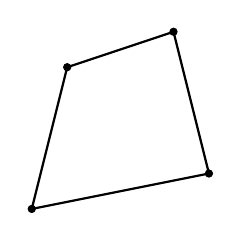
\begin{tikzpicture}[scale=0.45]

\draw[fill] (6,2) circle [radius=0.1];
\draw[fill] (5,6) circle [radius=0.1];
\draw[fill] (2,5) circle [radius=0.1];
\draw[fill] (1,1) circle [radius=0.1];
\draw[thick] (6,2) -- (5,6) -- (2,5) -- (1,1) -- (6,2);
\end{tikzpicture}
\end{center}
Una forma de abordar el problema es dividir
el cuadrilátero en dos triángulos mediante una recta
entre dos vértices opuestos:
\begin{center}
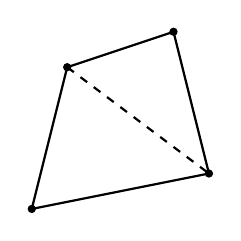
\begin{tikzpicture}[scale=0.45]

\draw[fill] (6,2) circle [radius=0.1];
\draw[fill] (5,6) circle [radius=0.1];
\draw[fill] (2,5) circle [radius=0.1];
\draw[fill] (1,1) circle [radius=0.1];

\draw[thick] (6,2) -- (5,6) -- (2,5) -- (1,1) -- (6,2);
\draw[dashed,thick] (2,5) -- (6,2);
\end{tikzpicture}
\end{center}
Después de esto, basta con sumar las áreas
de los triángulos.
El área de un triángulo se puede calcular,
por ejemplo, usando la \key{fórmula de Herón}
%\footnote{Heron de Alejandría (c. 10--70) fue un matemático griego.}
\[ \sqrt{s (s-a) (s-b) (s-c)},\]
donde $a$, $b$ y $c$ son las longitudes
de los lados del triángulo y
$s=(a+b+c)/2$.
\index{Heron's formula}

Esta es una forma posible de resolver el problema,
pero hay un escollo:
¿cómo dividir el cuadrilátero en triángulos?
Resulta que a veces no podemos simplemente elegir
dos vértices opuestos arbitrarios.
Por ejemplo, en la siguiente situación,
la línea de división está \emph{fuera} del cuadrilátero:
\begin{center}
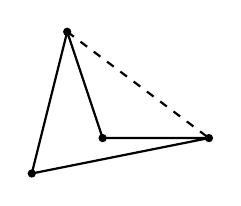
\begin{tikzpicture}[scale=0.45]

\draw[fill] (6,2) circle [radius=0.1];
\draw[fill] (3,2) circle [radius=0.1];
\draw[fill] (2,5) circle [radius=0.1];
\draw[fill] (1,1) circle [radius=0.1];
\draw[thick] (6,2) -- (3,2) -- (2,5) -- (1,1) -- (6,2);

\draw[dashed,thick] (2,5) -- (6,2);
\end{tikzpicture}
\end{center}
Sin embargo, otra forma de dibujar la línea funciona:
\begin{center}
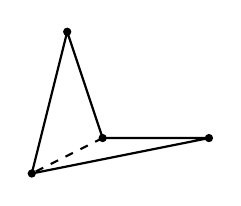
\begin{tikzpicture}[scale=0.45]

\draw[fill] (6,2) circle [radius=0.1];
\draw[fill] (3,2) circle [radius=0.1];
\draw[fill] (2,5) circle [radius=0.1];
\draw[fill] (1,1) circle [radius=0.1];
\draw[thick] (6,2) -- (3,2) -- (2,5) -- (1,1) -- (6,2);

\draw[dashed,thick] (3,2) -- (1,1);
\end{tikzpicture}
\end{center}
Es claro para un humano cuál de las líneas es la correcta
elección, pero la situación es difícil para una computadora.
                           
Sin embargo, resulta que podemos resolver el problema usando
otro método que es más conveniente para un programador.
Es decir, existe una fórmula general
\[x_1y_2-x_2y_1+x_2y_3-x_3y_2+x_3y_4-x_4y_3+x_4y_1-x_1y_4,\]
que calcula el área de un cuadrilátero
cuyos vértices son
$(x_1,y_1)$,
$(x_2,y_2)$,
$(x_3,y_3)$ y
$(x_4,y_4)$.
Esta fórmula es fácil de implementar, no hay casos especiales
y podemos incluso generalizar la fórmula
a \emph{todos} los polígonos.

\section{Números complejos}

\index{complex number}
\index{point}
\index{vector}

Un \key{número complejo} es un número de la forma $x+y i$,
donde $i = \sqrt{-1}$ es la \key{unidad imaginaria}.
Una interpretación geométrica de un número complejo es
que representa un punto bidimensional $(x,y)$
o un vector desde el origen hasta un punto $(x,y)$.

Por ejemplo, $4+2i$ corresponde a
el siguiente punto y vector:

\begin{center}
\begin{tikzpicture}[scale=0.45]

\draw[->,thick] (-5,0)--(5,0);
\draw[->,thick] (0,-5)--(0,5);

\draw[fill] (4,2) circle [radius=0.1];
\draw[->,thick] (0,0)--(4-0.1,2-0.1);

\node at (4,2.8) {$(4,2)$};
\end{tikzpicture}
\end{center}

\index{complex@\texttt{complex}}

La clase de número complejo de C++ \texttt{complex} es
útil para resolver problemas geométricos.
Usando la clase podemos representar puntos y vectores
como números complejos, y la clase contiene herramientas
que son útiles en geometría.

En el siguiente código, \texttt{C} es el tipo de
una coordenada y \texttt{P} es el tipo de un punto o un vector.
Además, el código define las macros \texttt{X} y \texttt{Y}
que se pueden usar para referirse a las coordenadas x e y.

\begin{lstlisting}
typedef long long C;
typedef complex<C> P;
#define X real()
#define Y imag()
\end{lstlisting}

Por ejemplo, el siguiente código define un punto $p=(4,2)$
y imprime sus coordenadas x e y:

\begin{lstlisting}
P p = {4,2};
cout << p.X << " " << p.Y << "\n"; // 4 2
\end{lstlisting}

El siguiente código define vectores $v=(3,1)$ y $u=(2,2)$,
y después calcula la suma $s=v+u$.

\begin{lstlisting}
P v = {3,1};
P u = {2,2};
P s = v+u;
cout << s.X << " " << s.Y << "\n"; // 5 3
\end{lstlisting}
En la práctica,
un tipo de coordenada adecuado es usualmente
\texttt{long long} (entero) o \texttt{long double}
(número real).
Es una buena idea usar enteros siempre que sea posible,
porque los cálculos con enteros son exactos.
Si se necesitan números reales,
se deben tener en cuenta los errores de precisión
al comparar números.
Una forma segura de comprobar si los números reales $a$ y $b$ son iguales
es compararlos usando $|a-b|<\epsilon$,
donde $\epsilon$ es un número pequeño (por ejemplo, $\epsilon=10^{-9}$).

\subsubsection*{Funciones}

En los siguientes ejemplos, el tipo de coordenada es
\texttt{long double}.

La función $\texttt{abs}(v)$ calcula la longitud
$|v|$ de un vector $v=(x,y)$
usando la fórmula $\sqrt{x^2+y^2}$.
La función también se puede usar para
calcular la distancia entre puntos
$(x_1,y_1)$ y $(x_2,y_2)$,
porque esa distancia es igual a la longitud
del vector $(x_2-x_1,y_2-y_1)$.

El siguiente código calcula la distancia
entre los puntos $(4,2)$ y $(3,-1)$:
\begin{lstlisting}
P a = {4,2};
P b = {3,-1};
cout << abs(b-a) << "\n"; // 3.16228
\end{lstlisting}

La función $\texttt{arg}(v)$ calcula el
ángulo de un vector $v=(x,y)$ con respecto al eje x.
La función da el ángulo en radianes,
donde $r$ radianes es igual a $180 r/\pi$ grados.
El ángulo de un vector que apunta hacia la derecha es 0,
y los ángulos disminuyen en el sentido de las agujas del reloj y aumentan
en sentido contrario a las agujas del reloj.

La función $\texttt{polar}(s,a)$ construye un vector
cuya longitud es $s$ y que apunta a un ángulo $a$.
Un vector se puede rotar por un ángulo $a$
multiplicándolo por un vector con longitud 1 y ángulo $a$.

El siguiente código calcula el ángulo de
el vector $(4,2)$, lo rota $1/2$ radianes
en sentido contrario a las agujas del reloj, y luego calcula el ángulo nuevamente:

\begin{lstlisting}
P v = {4,2};
cout << arg(v) << "\n"; // 0.463648
v *= polar(1.0,0.5);
cout << arg(v) << "\n"; // 0.963648
\end{lstlisting}

\section{Puntos y líneas}

\index{producto cruz}

El \key{producto cruz} $a \times b$ de vectores
$a=(x_1,y_1)$ y $b=(x_2,y_2)$ se calcula
usando la fórmula $x_1 y_2 - x_2 y_1$.
El producto cruz nos dice si $b$
gira a la izquierda (valor positivo), no gira (cero)
o gira a la derecha (valor negativo)
cuando se coloca directamente después de $a$.

La siguiente imagen ilustra los casos anteriores:
\begin{center}
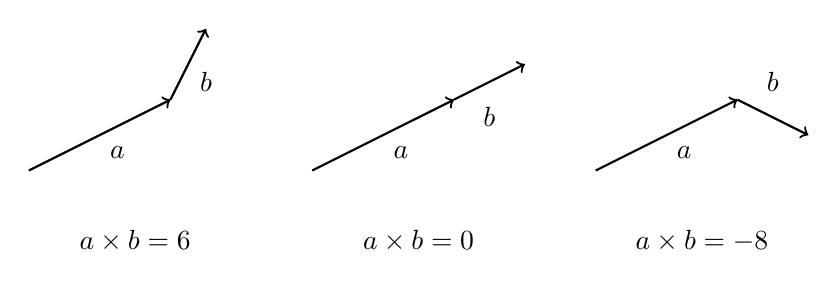
\begin{tikzpicture}[scale=0.45]

\draw[->,thick] (0,0)--(4,2);
\draw[->,thick] (4,2)--(4+1,2+2);

\node at (2.5,0.5) {$a$};
\node at (5,2.5) {$b$};

\node at (3,-2) {$a \times b = 6$};

\draw[->,thick] (8+0,0)--(8+4,2);
\draw[->,thick] (8+4,2)--(8+4+2,2+1);

\node at (8+2.5,0.5) {$a$};
\node at (8+5,1.5) {$b$};

\node at (8+3,-2) {$a \times b = 0$};

\draw[->,thick] (16+0,0)--(16+4,2);
\draw[->,thick] (16+4,2)--(16+4+2,2-1);

\node at (16+2.5,0.5) {$a$};
\node at (16+5,2.5) {$b$};

\node at (16+3,-2) {$a \times b = -8$};
\end{tikzpicture}
\end{center}

\noindent
Por ejemplo, en el primer caso
$a=(4,2)$ y $b=(1,2)$.
El siguiente código calcula el producto cruz
usando la clase \texttt{complex}:

\begin{lstlisting}
P a = {4,2};
P b = {1,2};
C p = (conj(a)*b).Y; // 6
\end{lstlisting}

El código anterior funciona, porque
la función \texttt{conj} niega la coordenada y
de un vector,
y cuando los vectores $(x_1,-y_1)$ y $(x_2,y_2)$
se multiplican, la coordenada y
del resultado es $x_1 y_2 - x_2 y_1$.

\subsubsection{Ubicación del punto}

Los productos cruzados se pueden usar para probar
si un punto está ubicado a la izquierda o derecha
de una línea.
Asumimos que la línea pasa por los puntos
$s_1$ y $s_2$, estamos mirando desde $s_1$
a $s_2$ y el punto es $p$.

Por ejemplo, en la siguiente imagen,
$p$ está a la izquierda de la línea:
\begin{center}
\begin{tikzpicture}[scale=0.45]
\draw[dashed,thick,->] (0,-3)--(12,6);
\draw[fill] (4,0) circle [radius=0.1];
\draw[fill] (8,3) circle [radius=0.1];
\draw[fill] (5,3) circle [radius=0.1];
\node at (4,-1) {$s_1$};
\node at (8,2) {$s_2$};
\node at (5,4) {$p$};
\end{tikzpicture}
\end{center}

El producto cruz $(p-s_1) \times (p-s_2)$
nos dice la ubicación del punto $p$.
Si el producto cruz es positivo,
$p$ está ubicado a la izquierda,
y si el producto cruz es negativo,
$p$ está ubicado a la derecha.
Finalmente, si el producto cruz es cero,
los puntos $s_1$, $s_2$ y $p$ están en la misma línea.

\subsubsection{Intersección de segmentos de línea}

\index{intersección de segmentos de línea}

A continuación, consideramos el problema de probar
si dos segmentos de línea
$ab$ y $cd$ se cruzan. Los posibles casos son:
\textit{Caso 1:}
Los segmentos de línea están en la misma línea
y se superponen entre sí.
En este caso, hay un número infinito de
puntos de intersección.
Por ejemplo, en la siguiente imagen,
todos los puntos entre $c$ y $b$ son
puntos de intersección:
\begin{center}
\begin{tikzpicture}[scale=0.9]
\draw (1.5,1.5)--(6,3);
\draw (0,1)--(4.5,2.5);
\draw[fill] (0,1) circle [radius=0.05];
\node at (0,0.5) {$a$};
\draw[fill] (1.5,1.5) circle [radius=0.05];
\node at (6,2.5) {$d$};
\draw[fill] (4.5,2.5) circle [radius=0.05];
\node at (1.5,1) {$c$};
\draw[fill] (6,3) circle [radius=0.05];
\node at (4.5,2) {$b$};
\end{tikzpicture}
\end{center}

En este caso, podemos usar productos cruzados para
comprobar si todos los puntos están en la misma línea.
Después de esto, podemos ordenar los puntos y verificar
si los segmentos de línea se superponen entre sí.

\textit{Caso 2:}
Los segmentos de línea tienen un vértice común
que es el único punto de intersección.
Por ejemplo, en la siguiente imagen el
punto de intersección es $b=c$:

\begin{center}
\begin{tikzpicture}[scale=0.9]
\draw (0,0)--(4,2);
\draw (4,2)--(6,1);
\draw[fill] (0,0) circle [radius=0.05];
\draw[fill] (4,2) circle [radius=0.05];
\draw[fill] (6,1) circle [radius=0.05];

\node at (0,0.5) {$a$};
\node at (4,2.5) {$b=c$};
\node at (6,1.5) {$d$};
\end{tikzpicture}
\end{center}

Este caso es fácil de comprobar, porque
solo hay cuatro posibilidades
para el punto de intersección:
$a=c$, $a=d$, $b=c$ y $b=d$.

\textit{Caso 3:}
Hay exactamente un punto de intersección
que no es un vértice de ningún segmento de línea.
En la siguiente imagen, el punto $p$
es el punto de intersección:
\begin{center}
\begin{tikzpicture}[scale=0.9]
\draw (0,1)--(6,3);
\draw (2,4)--(4,0);
\draw[fill] (0,1) circle [radius=0.05];
\node at (0,0.5) {$c$};
\draw[fill] (6,3) circle [radius=0.05];
\node at (6,2.5) {$d$};
\draw[fill] (2,4) circle [radius=0.05];
\node at (1.5,3.5) {$a$};
\draw[fill] (4,0) circle [radius=0.05];
\node at (4,-0.4) {$b$};
\draw[fill] (3,2) circle [radius=0.05];
\node at (3,1.5) {$p$};
\end{tikzpicture}
\end{center}

En este caso, los segmentos de línea se intersecan
exactamente cuando ambos puntos $c$ y $d$ son
en lados diferentes de una línea a través de $a$ y $b$,
y los puntos $a$ y $b$ están en diferentes
lados de una línea a través de $c$ y $d$.
Podemos usar productos cruzados para comprobar esto.

\subsubsection{Distancia de un punto a una línea}

Otra característica de los productos cruzados es que
el área de un triángulo se puede calcular
usando la fórmula
\[\frac{| (a-c) \times (b-c) |}{2},\]
donde $a$, $b$ y $c$ son los vértices del triángulo.
Usando este hecho, podemos derivar una fórmula
para calcular la distancia más corta entre un punto y una línea.
Por ejemplo, en la siguiente imagen $d$ es la
distancia más corta entre el punto $p$ y la línea
que está definida por los puntos $s_1$ y $s_2$:
\begin{center}
\begin{tikzpicture}[scale=0.75]
\draw (-2,-1)--(6,3);
\draw[dashed] (1,4)--(2.40,1.2);
\node at (0,-0.5) {$s_1$};
\node at (4,1.5) {$s_2$};
\node at (0.5,4) {$p$};
\node at (2,2.7) {$d$};
\draw[fill] (0,0) circle [radius=0.05];
\draw[fill] (4,2) circle [radius=0.05];
\draw[fill] (1,4) circle [radius=0.05];
\end{tikzpicture}
\end{center}

El área del triángulo cuyos vértices son
$s_1$, $s_2$ y $p$ se puede calcular de dos maneras:
es tanto
$\frac{1}{2} |s_2-s_1| d$ como
$\frac{1}{2} ((s_1-p) \times (s_2-p))$.
Por lo tanto, la distancia más corta es
\[ d = \frac{(s_1-p) \times (s_2-p)}{|s_2-s_1|} .\]

\subsubsection{Punto dentro de un polígono}

Consideremos ahora el problema de
probar si un punto está ubicado dentro o fuera
de un polígono.
Por ejemplo, en la siguiente imagen el punto $a$
está dentro del polígono y el punto $b$ está fuera
del polígono.

\begin{center}
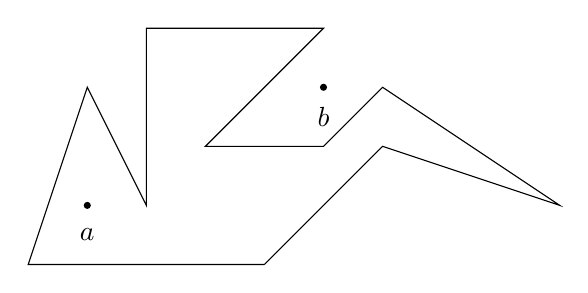
\begin{tikzpicture}[scale=0.75]
%\draw (0,0)--(2,-2)--(3,1)--(5,1)--(2,3)--(1,2)--(-1,2)--(1,4)--(-2,4)--(-2,1)--(-3,3)--(-4,0)--(0,0);
\draw (0,0)--(2,2)--(5,1)--(2,3)--(1,2)--(-1,2)--(1,4)--(-2,4)--(-2,1)--(-3,3)--(-4,0)--(0,0);

\draw[fill] (-3,1) circle [radius=0.05];
\node at (-3,0.5) {$a$};
\draw[fill] (1,3) circle [radius=0.05];
\node at (1,2.5) {$b$};
\end{tikzpicture}
\end{center}

Una forma conveniente de resolver el problema es
enviar un \emph{rayo} desde el punto a una dirección arbitraria
y calcular el número de veces que toca
el límite del polígono.
Si el número es impar,
el punto está dentro del polígono,
y si el número es par,
el punto está fuera del polígono.

\begin{samepage}
Por ejemplo, podríamos enviar los siguientes rayos:
\begin{center}
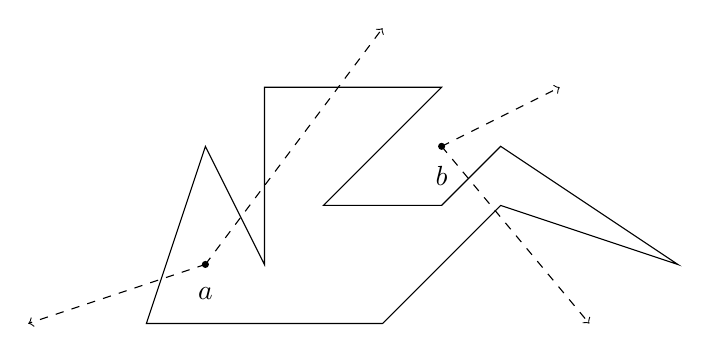
\begin{tikzpicture}[scale=0.75]
\draw (0,0)--(2,2)--(5,1)--(2,3)--(1,2)--(-1,2)--(1,4)--(-2,4)--(-2,1)--(-3,3)--(-4,0)--(0,0);

\draw[fill] (-3,1) circle [radius=0.05];
\node at (-3,0.5) {$a$};
\draw[fill] (1,3) circle [radius=0.05];
\node at (1,2.5) {$b$};

\draw[dashed,->] (-3,1)--(-6,0);
\draw[dashed,->] (-3,1)--(0,5);

\draw[dashed,->] (1,3)--(3.5,0);
\draw[dashed,->] (1,3)--(3,4);
\end{tikzpicture}
\end{center}
\end{samepage}


Los rayos desde $a$ tocan 1 y 3 veces
el límite del polígono,
por lo que $a$ está dentro del polígono.
Correspondientemente, los rayos desde $b$
tocan 0 y 2 veces el límite del polígono,
por lo que $b$ está fuera del polígono.

\section{Área del polígono}

Una fórmula general para calcular el área
de un polígono, a veces llamada la fórmula del \key{cordón de zapatos},
es la siguiente: \index{fórmula del cordón de zapatos}
\[\frac{1}{2} |\sum_{i=1}^{n-1} (p_i \times p_{i+1})| =
\frac{1}{2} |\sum_{i=1}^{n-1} (x_i y_{i+1} - x_{i+1} y_i)|, \]
Aquí los vértices son
$p_1=(x_1,y_1)$, $p_2=(x_2,y_2)$, $\ldots$, $p_n=(x_n,y_n)$
en tal orden que
$p_i$ y $p_{i+1}$ son vértices adyacentes en el límite
del polígono,
y el primer y último vértice es el mismo, es decir, $p_1=p_n$.

Por ejemplo, el área del polígono
\begin{center}
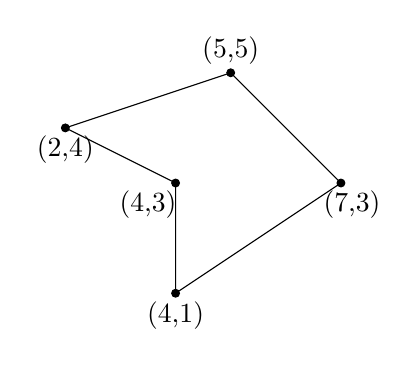
\begin{tikzpicture}[scale=0.7]
\filldraw (4,1.4) circle (2pt);
\filldraw (7,3.4) circle (2pt);
\filldraw (5,5.4) circle (2pt);
\filldraw (2,4.4) circle (2pt);
\filldraw (4,3.4) circle (2pt);
\node (1) at (4,1) {(4,1)};
\node (2) at (7.2,3) {(7,3)};
\node (3) at (5,5.8) {(5,5)};
\node (4) at (2,4) {(2,4)};
\node (5) at (3.5,3) {(4,3)};
\path[draw] (4,1.4) -- (7,3.4) -- (5,5.4) -- (2,4.4) -- (4,3.4) -- (4,1.4);
\end{tikzpicture}
\end{center}
es
\[\frac{|(2\cdot5-5\cdot4)+(5\cdot3-7\cdot5)+(7\cdot1-4\cdot3)+(4\cdot3-4\cdot1)+(4\cdot4-2\cdot3)|}{2} = 17/2.\]

La idea de la fórmula es recorrer los trapecios
cuyo un lado es un lado del polígono,
y otro lado yace en la línea horizontal $y=0$.
Por ejemplo:
\begin{center}
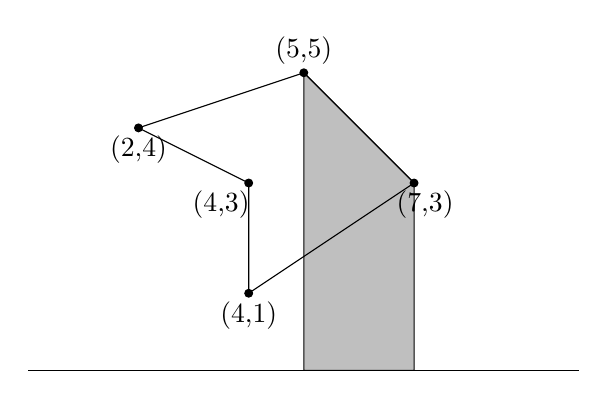
\begin{tikzpicture}[scale=0.7]
\path[draw,fill=lightgray] (5,5.4) -- (7,3.4) -- (7,0) -- (5,0) -- (5,5.4);
\filldraw (4,1.4) circle (2pt);
\filldraw (7,3.4) circle (2pt);
\filldraw (5,5.4) circle (2pt);
\filldraw (2,4.4) circle (2pt);
\filldraw (4,3.4) circle (2pt);
\node (1) at (4,1) {(4,1)};
\node (2) at (7.2,3) {(7,3)};
\node (3) at (5,5.8) {(5,5)};
\node (4) at (2,4) {(2,4)};
\node (5) at (3.5,3) {(4,3)};
\path[draw] (4,1.4) -- (7,3.4) -- (5,5.4) -- (2,4.4) -- (4,3.4) -- (4,1.4);
\draw (0,0) -- (10,0);
\end{tikzpicture}
\end{center}
El área de tal trapecio es
\[(x_{i+1}-x_{i}) \frac{y_i+y_{i+1}}{2},\]
donde los vértices del polígono son $p_i$ y $p_{i+1}$.
Si $x_{i+1}>x_{i}$, el área es positiva,
y si $x_{i+1}<x_{i}$, el área es negativa.

El área del polígono es la suma de áreas de
todos los trapecios, lo que produce la fórmula
\[|\sum_{i=1}^{n-1} (x_{i+1}-x_{i}) \frac{y_i+y_{i+1}}{2}| =
\frac{1}{2} |\sum_{i=1}^{n-1} (x_i y_{i+1} - x_{i+1} y_i)|.\]

Tenga en cuenta que se toma el valor absoluto de la suma,
porque el valor de la suma puede ser positivo o negativo,
dependiendo de si caminamos en sentido horario o antihorario
a lo largo del límite del polígono.

\subsubsection{Teorema de Pick}

\index{Teorema de Pick}

El \key{Teorema de Pick} proporciona otra forma de calcular
el área de un polígono siempre que todos los vértices
del polígono tengan coordenadas enteras.
De acuerdo con el teorema de Pick, el área del polígono es
\[ a + b/2 -1,\]
donde $a$ es el número de puntos enteros dentro del polígono
y $b$ es el número de puntos enteros en el límite del polígono.

Por ejemplo, el área del polígono
\begin{center}
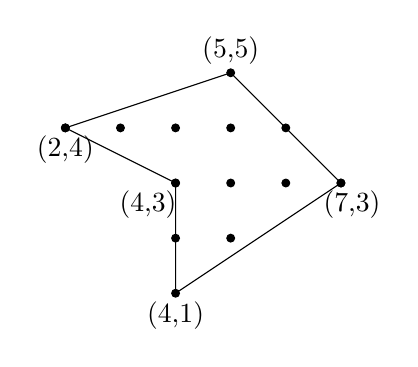
\begin{tikzpicture}[scale=0.7]
\filldraw (4,1.4) circle (2pt);
\filldraw (7,3.4) circle (2pt);
\filldraw (5,5.4) circle (2pt);
\filldraw (2,4.4) circle (2pt);
\filldraw (4,3.4) circle (2pt);
\node (1) at (4,1) {(4,1)};
\node (2) at (7.2,3) {(7,3)};
\node (3) at (5,5.8) {(5,5)};
\node (4) at (2,4) {(2,4)};
\node (5) at (3.5,3) {(4,3)};
\path[draw] (4,1.4) -- (7,3.4) -- (5,5.4) -- (2,4.4) -- (4,3.4) -- (4,1.4);

\filldraw (2,4.4) circle (2pt);
\filldraw (3,4.4) circle (2pt);
\filldraw (4,4.4) circle (2pt);
\filldraw (5,4.4) circle (2pt);
\filldraw (6,4.4) circle (2pt);

\filldraw (4,3.4) circle (2pt);
\filldraw (5,3.4) circle (2pt);
\filldraw (6,3.4) circle (2pt);
\filldraw (7,3.4) circle (2pt);

\filldraw (4,2.4) circle (2pt);
\filldraw (5,2.4) circle (2pt);
\end{tikzpicture}
\end{center}
es $6+7/2-1=17/2$.

\section{Funciones de distancia}

\index{función de distancia}
\index{distancia euclidiana}
\index{distancia de Manhattan}

Una \key{función de distancia} define la distancia entre
dos puntos.
La función de distancia habitual es la
\key{distancia euclidiana} donde la distancia entre
los puntos $(x_1,y_1)$ y $(x_2,y_2)$ es
\[\sqrt{(x_2-x_1)^2+(y_2-y_1)^2}.\]
Una función de distancia alternativa es la
\key{distancia de Manhattan}
donde la distancia entre los puntos
$(x_1,y_1)$ y $(x_2,y_2)$ es
\[|x_1-x_2|+|y_1-y_2|.\]
\begin{samepage}
Por ejemplo, considere la siguiente imagen:
\begin{center}
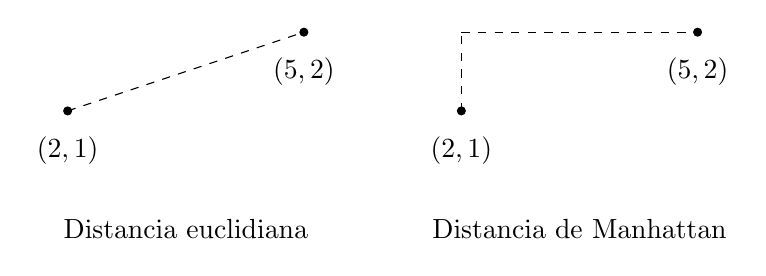
\begin{tikzpicture}

\draw[fill] (2,1) circle [radius=0.05];
\draw[fill] (5,2) circle [radius=0.05];

\node at (2,0.5) {$(2,1)$};
\node at (5,1.5) {$(5,2)$};

\draw[dashed] (2,1) -- (5,2);

\draw[fill] (5+2,1) circle [radius=0.05];
\draw[fill] (5+5,2) circle [radius=0.05];

\node at (5+2,0.5) {$(2,1)$};
\node at (5+5,1.5) {$(5,2)$};

\draw[dashed] (5+2,1) -- (5+2,2);
\draw[dashed] (5+2,2) -- (5+5,2);

\node at (3.5,-0.5) {Distancia euclidiana};
\node at (5+3.5,-0.5) {Distancia de Manhattan};
\end{tikzpicture}
\end{center}
\end{samepage}
La distancia euclidiana entre los puntos es
\[\sqrt{(5-2)^2+(2-1)^2}=\sqrt{10}\]
y la distancia de Manhattan es
\[|5-2|+|2-1|=4.\]
La siguiente imagen muestra regiones que están dentro de una distancia de 1
del punto central, usando las distancias euclidiana y de Manhattan:
\begin{center}
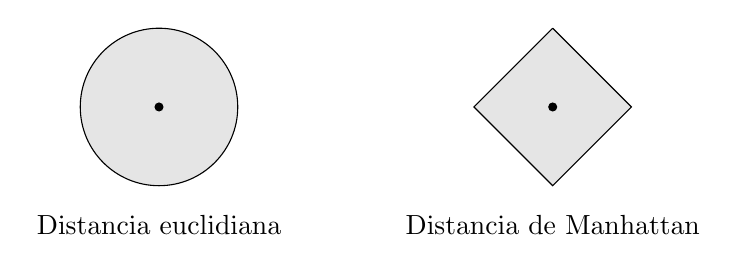
\begin{tikzpicture}

\draw[fill=gray!20] (0,0) circle [radius=1];
\draw[fill] (0,0) circle [radius=0.05];

\node at (0,-1.5) {Distancia euclidiana};

\draw[fill=gray!20] (5+0,1) -- (5-1,0) -- (5+0,-1) -- (5+1,0) -- (5+0,1);
\draw[fill] (5,0) circle [radius=0.05];
\node at (5,-1.5) {Distancia de Manhattan};
\end{tikzpicture}
\end{center}

\subsubsection{Rotación de coordenadas}

Algunos problemas son más fáciles de resolver si
se usan distancias de Manhattan en lugar de distancias euclidianas.
Como ejemplo, considere un problema donde se nos dan
$n$ puntos en el plano bidimensional
y nuestra tarea es calcular la distancia de Manhattan máxima
entre dos puntos cualesquiera.

Por ejemplo, considere el siguiente conjunto de puntos:
\begin{center}
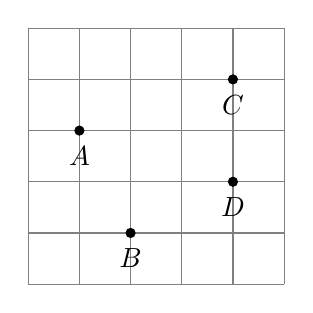
\begin{tikzpicture}[scale=0.65]
\draw[color=gray] (-1,-1) grid (4,4);

\filldraw (0,2) circle (2.5pt);
\filldraw (3,3) circle (2.5pt);
\filldraw (1,0) circle (2.5pt);
\filldraw (3,1) circle (2.5pt);

\node at (0,1.5) {$A$};
\node at (3,2.5) {$C$};
\node at (1,-0.5) {$B$};
\node at (3,0.5) {$D$};
\end{tikzpicture}
\end{center}
La distancia de Manhattan máxima es 5
entre los puntos $B$ y $C$:
\begin{center}
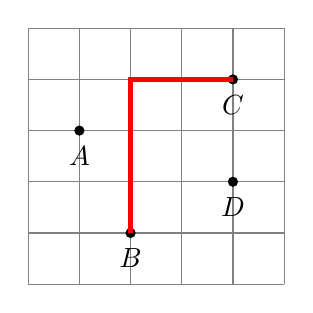
\begin{tikzpicture}[scale=0.65]
\draw[color=gray] (-1,-1) grid (4,4);

\filldraw (0,2) circle (2.5pt);
\filldraw (3,3) circle (2.5pt);
\filldraw (1,0) circle (2.5pt);
\filldraw (3,1) circle (2.5pt);

\node at (0,1.5) {$A$};
\node at (3,2.5) {$C$};
\node at (1,-0.5) {$B$};
\node at (3,0.5) {$D$};

\path[draw=red,thick,line width=2pt] (1,0) -- (1,3) -- (3,3);
\end{tikzpicture}
\end{center}

Una técnica útil relacionada con las distancias de Manhattan
es rotar todas las coordenadas 45 grados para que
un punto $(x,y)$ se convierta en $(x+y,y-x)$.
Por ejemplo, después de rotar los puntos anteriores,
el resultado es:

\begin{center}
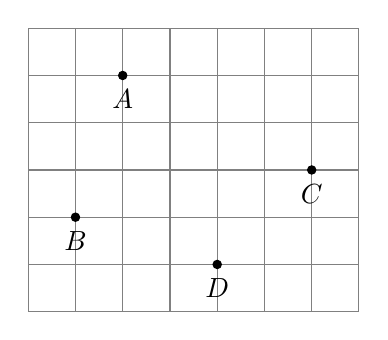
\begin{tikzpicture}[scale=0.6]
\draw[color=gray] (0,-3) grid (7,3);

\filldraw (2,2) circle (2.5pt);
\filldraw (6,0) circle (2.5pt);
\filldraw (1,-1) circle (2.5pt);
\filldraw (4,-2) circle (2.5pt);

\node at (2,1.5) {$A$};
\node at (6,-0.5) {$C$};
\node at (1,-1.5) {$B$};
\node at (4,-2.5) {$D$};
\end{tikzpicture}
\end{center}
Y la distancia máxima es la siguiente:
\begin{center}
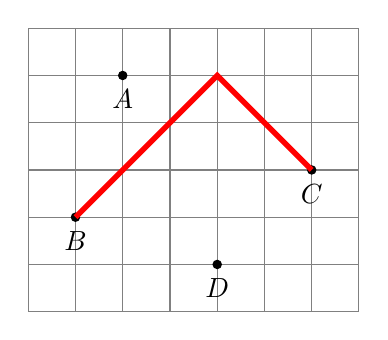
\begin{tikzpicture}[scale=0.6]
\draw[color=gray] (0,-3) grid (7,3);

\filldraw (2,2) circle (2.5pt);
\filldraw (6,0) circle (2.5pt);
\filldraw (1,-1) circle (2.5pt);
\filldraw (4,-2) circle (2.5pt);

\node at (2,1.5) {$A$};
\node at (6,-0.5) {$C$};
\node at (1,-1.5) {$B$};
\node at (4,-2.5) {$D$};

\path[draw=red,thick,line width=2pt] (1,-1) -- (4,2) -- (6,0);
\end{tikzpicture}
\end{center}

Considere dos puntos $p_1=(x_1,y_1)$ y $p_2=(x_2,y_2)$ cuyas coordenadas
giradas son $p'_1=(x'_1,y'_1)$ y $p'_2=(x'_2,y'_2)$.
Ahora hay dos formas de expresar la distancia de Manhattan
entre $p_1$ y $p_2$:
\[|x_1-x_2|+|y_1-y_2| = \max(|x'_1-x'_2|,|y'_1-y'_2|)\]

Por ejemplo, si $p_1=(1,0)$ y $p_2=(3,3)$,
las coordenadas giradas son $p'_1=(1,-1)$ y $p'_2=(6,0)$
y la distancia de Manhattan es
\[|1-3|+|0-3| = \max(|1-6|,|-1-0|) = 5.\]

Las coordenadas giradas proporcionan una forma sencilla
de operar con distancias de Manhattan, porque podemos
considerar las coordenadas x e y por separado.
Para maximizar la distancia de Manhattan entre dos puntos,
deberíamos encontrar dos puntos cuyas
coordenadas giradas maximicen el valor de
\[\max(|x'_1-x'_2|,|y'_1-y'_2|).\]
Esto es fácil, porque o la diferencia horizontal o la vertical
de las coordenadas giradas tiene que ser máxima.


